
\chapter{Lineare Algebra}
\section{Matrizen}
\subsection{Definitionen}
\begin{Definition}[Transponierte Matrix]%
\index{transponierte Matrix}
Sei $R$ ein Ring und $A\in R^{m\times n}$ eine Matrix.
Die Matrix $A^T\in R^{n\times m}$ mit $(A^T)_{ij} := A_{ji}$
heißt Transponierte von $A$.
\end{Definition}

\begin{Definition}[Konjugierte Matrix]%
\index{konjugierte Matrix}
Sei $A\in\C^{m\times n}$. Die Matrix $\overline A$ mit
$(\overline A)_{ij} := \overline{A_{ij}}$
heißt konjugierte Matrix zu $A$. Mit $\overline{A_{ij}}$ ist
die Konjugation der komplexen Zahl $A_{ij}$ gemeint.
\end{Definition}

\begin{Definition}[Adjungierte Matrix]%
\index{adjungierte Matrix}
Sei $A\in\C^{m\times n}$. Die Adjungierte zu $A$ ist
definiert als $A^H:=(\overline A)^T$, d.\,h.
die Transponierte der konjugierten Matrix zu $A$.
\end{Definition}

\begin{Definition}[Inverse Matrix]%
\label{matrix-inv}\index{inverse Matrix}
Sei $K$ ein Körper und $A\in K^{n\times n}$ eine quadratische
Matrix. Man nennt $A$ invertierbar, wenn es eine Matrix $B$ gibt,
mit $AB=BA=E_n$, wobei $E_n$ die Einheitsmatrix ist. Die Matrix
$A^{-1}:=B$ heißt dann inverse Matrix zu $A$.
\end{Definition}

\subsection{Rechenregeln}

\begin{Korollar}\label{matrix-mul-tp}
Sei $R$ ein kommutativer Ring. Für Matrizen $A\in R^{m\times n}$ und
$B\in R^{n\times p}$ gilt
\[(AB)^T = B^T A^T.\]
\end{Korollar}
\begin{Beweis} Es gilt:
\begin{align}
(AB)^T &= \bigg(\sum_{k=1}^n A_{ik}B_{kj}\bigg)^T
= \bigg(\sum_{k=1}^n A_{jk}B_{ki}\bigg)
= \bigg(\sum_{k=1}^n B_{ki} A_{jk}\bigg)\\
&= \bigg(\sum_{k=1}^n (B^T)_{ik} (A^T)_{kj}\bigg)
= B^T A^T.\;\qedsymbol
\end{align}
\end{Beweis}

\begin{Korollar}
Sei $A\in K^{n\times n}$ eine invertierbare Matrix. Dann ist auch
$A^T$ invertierbar und es gilt $(A^{-1})^T = (A^T)^{-1}$.
\end{Korollar}
\begin{Beweis}
Aus $E=A^{-1}A=AA^{-1}$ und Korollar \ref{matrix-mul-tp} folgt
\begin{equation}
E = E^T = (A^{-1}A)^T = A^T (A^{-1})^T = (AA^{-1})^T = (A^{-1})^T A^T.
\end{equation}
Dann muss $A^T$ nach Def. \ref{matrix-inv} die inverse Matrix
zu $(A^{-1})^T$ sein.\;\qedsymbol
\end{Beweis}

\newpage
\begin{Korollar}\label{Verschiebungseigenschaft}
Sei $v\in\R^n$ und $w\in\R^m$. Sei $A\in\R^{m\times n}$. Es gilt
$\langle Av,w\rangle = \langle v,A^Tw\rangle$,
wobei links das Standardskalarprodukt auf dem $\R^m$ und
rechts das auf dem $\R^n$ ausgewertet wird.
\end{Korollar}
\begin{Beweis}
Identifiziert man die Vektoren $x,y\in\R^k$ mit den
Matrizen $x,y\in\R^{k\times 1}$, dann
ist $\langle x,y\rangle = x^T y$. Gemäß Korollar
\ref{matrix-mul-tp} darf man rechnen:
\[\langle Av,w\rangle
= (Av)^T w = v^T A^T w = \langle v,A^Tw\rangle.\;\qedsymbol\]
\end{Beweis}

\subsection{Rechenregeln für komplexe Matrizen}
\begin{Korollar}\label{matrix-mul-conj}
Für Matrizen $A\in\C^{m\times n}$ und $B\in\C^{n\times p}$ gilt
\[\overline{AB} = \overline A\cdot\overline B\]
\end{Korollar}
\begin{Beweis}
Es gilt
\begin{align*}
\overline{AB}
&= \overline{\bigg(\sum_{k=1}^n A_{ik}B_{kj}\bigg)}
= \bigg(\sum_{k=1}^n \overline{A_{ik}B_{kj}}\bigg)
= \bigg(\sum_{k=1}^n \overline{A_{ik}}\cdot\overline{B_{kj}}\bigg)
= \bigg(\sum_{k=1}^n (\overline A)_{ik}(\overline B)_{kj}\bigg)
= \overline A\cdot\overline B.\;\qedsymbol
\end{align*}
\end{Beweis}

\begin{Korollar}\label{matrix-mul-tp-conj}
Für Matrizen $A\in\C^{m\times n}$ und $B\in\C^{n\times p}$ gilt
\[(AB)^H = B^H A^H.\]
\end{Korollar}
\begin{Beweis}
Gemäß Korollar \ref{matrix-mul-conj} und \ref{matrix-mul-tp} gilt
\[(AB)^H = (\overline{AB})^T = (\overline A\cdot\overline B)^T
= (\overline B)^T(\overline A)^T = B^H A^H.\]
\end{Beweis}

\begin{Korollar}\label{Verschiebungseigenschaft-komplex}
Sei $v\in\C^n$ und $w\in\C^m$. Sei $A\in\C^{m\times n}$.
Es gilt $\langle Av,w\rangle = \langle v,A^H w\rangle$,
wobei links das Standardskalarprodukt auf dem $\C^m$ ausgewertet
wird und rechts das auf dem $\C^n$.
\end{Korollar}
\begin{Beweis}
Identifiziert man die Vektoren $x,y\in\C^k$ mit den Matrizen
$x,y\in\C^{k\times 1}$, dann gilt $\langle x,y\rangle = x^H y$.
Gemäß Korollar \ref{matrix-mul-tp-conj} darf man rechnen
\[\langle Av,w\rangle = (Av)^H w = v^H A^H w
= \langle v,A^Hw\rangle.\;\qedsymbol\]
\end{Beweis}

%\newpage
\section{Eigenwerte}

\begin{Satz}
Gegeben sei eine quadratische Matrix $A\in\R^{n\times n}$.
Dann ist die Matrix $M=A^T A$ symmetrisch und besitzt nur
nichtnegative Eigenwerte, speziell bei $\det(A)\ne 0$ nur positive.
\end{Satz}

\begin{Beweis}
Gemäß Satz \ref{matrix-mul-tp} gilt
\begin{equation}
M^T = (A^T A)^T = A^T (A^T)^T = A^T A = M.
\end{equation}
Ist nun $\lambda$ ein Eigenwert von $M$ und $v$ ein Eigenvektor dazu,
dann gilt $Mv=\lambda v$. Unter Anwendung von Korollar
\ref{Verschiebungseigenschaft} folgt daraus
\begin{equation}
\lambda |v|^2 = \langle\lambda v,v\rangle
= \langle Mv,v\rangle = \langle A^T Av,v\rangle
= \langle Av,Av\rangle = |Av|^2\ge 0.
\end{equation}
Ergo ist $\lambda|v|^2\ge 0$. Unter der Voraussetzung $v\ne 0$ ist
$|v|>0$. Dann muss auch $\lambda\ge 0$ sein. Wenn nun $\det(A)\ne 0$
ist, also $A$ eine reguläre Matrix, dann hat $A$ trivialen Kern,
also $Av=0$ nur im Fall $v=0$. Da $v\ne 0$ vorausgesetzt wurde,
muss auch $Av\ne 0$, und damit $|Av|>0$ sein. Dann ist auch
$\lambda>0$. Alternativ folgt $\lambda>0$ daraus, dass $\det(A)$
das Produkt der Eigenwerte ist.\;\qedsymbol
\end{Beweis}

\begin{Satz}
Gegeben sei eine Matrix $A\in\C^{m\times n}$.
Dann ist die Matrix $M=A^H A$ hermitisch und besitzt nur
nichtnegative reelle Eigenwerte.
\end{Satz}
\begin{Beweis}
Gemäß Satz \ref{matrix-mul-tp-conj} gilt
\begin{equation}
M^H = (A^H A)^H = A^H (A^H)^H = A^H A = M.
\end{equation}
Ist nun $\lambda$ ein Eigenwert von $M$ und $v$ ein Eigenvektor dazu,
dann gilt $Mv=\lambda v$. Unter Anwendung von Korollar
\ref{Verschiebungseigenschaft-komplex} folgt daraus
\begin{equation}
\lambda |v|^2 = \langle\lambda v,v\rangle
= \langle Mv,v\rangle = \langle A^H Av,v\rangle
= \langle Av,Av\rangle = |Av|^2\ge 0.
\end{equation}
Ergo ist $\lambda|v|^2\ge 0$. Unter der Voraussetzung $v\ne 0$
ist $|v|>0$. Dann muss auch $\lambda\ge 0$ sein.\;\qedsymbol
\end{Beweis}

\begin{Definition}[Unitäre Matrix]\index{unitäre Matrix}\newlinefirst
Eine quadratische Matrix $A$ heißt unitär, wenn $A^H A=E$ gilt.
\end{Definition}

\begin{Korollar}
Ist $A$ unitär, dann gilt $|Av|=|v|$ für jeden Vektor $v$.
\end{Korollar}
\begin{Beweis}
Laut Korollar \ref{Verschiebungseigenschaft-komplex} gilt
\[|Av|^2 = \langle Av,Av\rangle = \langle v,A^H Av\rangle
= \langle v,Ev\rangle = \langle v,v\rangle = |v|^2.\]
Radizieren ergibt $|Av|=|v|$.\;\qedsymbol
\end{Beweis}

\begin{Korollar}
Für jeden Eigenwert $\lambda$ einer unitären Matrix gilt $|\lambda|=1$.
\end{Korollar}
\begin{Beweis}
Sei $v$ ein Eigenvektor zum Eigenwert $\lambda$. Laut Korollar
\ref{Verschiebungseigenschaft-komplex} ist dann
\[|v|^2 = \langle v,v\rangle = \langle v,Ev\rangle
= \langle v,A^H Av\rangle = \langle Av,Av\rangle
= |Av|^2 = |\lambda v|^2
= |\lambda|^2 |v|^2.\]
Daher ist $|\lambda|^2=1$, und wegen $|\lambda|\ge 0$ folglich $|\lambda|=1$.\;\qedsymbol
\end{Beweis}



\newpage
\subsection{Quadratische Matrizen}
\begin{Satz}
Sei
\[I:=\begin{bmatrix}
0 & -1\\
1 & 0
\end{bmatrix},\quad
aE+bI = a\begin{bmatrix}1 & 0\\ 0 & 1\end{bmatrix}
+b\begin{bmatrix}0 & -1\\ 1 & 0\end{bmatrix}
=
\begin{bmatrix}
a & -b\\
b & a
\end{bmatrix}.\]
Die Menge $M := \{aE+bI\mid a,b\in\R\}$ bildet bezüglich
Matrizenaddition und Matrizenmultiplikation einen
Körper $(M,+,\cdot)$. Die Abbildung
\[\Phi\colon\C\to M,\quad \Phi(a+b\ui):= aE+bI\]
ist ein Isomorphismus zwischen Körpern.
\end{Satz}
\begin{Beweis}
Bei $(M,+)$ handelt es sich um eine Untergruppe der
kommutativen Gruppe $(\R^{2\times 2},+)$, denn gemäß
\begin{equation}\label{eq:matrix-repr-complex-add}
(aE+bI)+(cE+dI) = (a+b)E+(b+d)I \in M
\end{equation}
und
\begin{equation}
-(aE+bI) = (-a)E+(-b)I\in M
\end{equation}
ist das Untergruppenkriterium erfüllt. Die Abgeschlossenheit
bezüglich Multiplikation:
\begin{equation}\label{eq:matrix-repr-complex-mul}
\begin{split}
&(aE+bI)(cE+dI) = aEcE+aEdI+bIcE+bIdI\\
&= acE+adI+bcI+bdI^2
= (ac-bd)E+(ad+bc)I \in M.
\end{split}
\end{equation}
Das Kommutativgesetz:
\begin{equation}
\begin{split}
&(aE+bI)(cE+dI) = (ac-bd)E+(ad+bc)I\\
&= (ca-db)E+(cb+da)I = (cE+dI)(aE+bI).
\end{split}
\end{equation}
Das Assoziativgesetz ist für Matrizen allgemeingültig. Das multiplikativ
neutrale Element ist die Einheitsmatrix $E$. Wird nun $aE+bI\ne 0$
vorausgesetzt, dann ist $a\ne 0\lor b\ne 0$. Daher ist
$\det(aE+bI)=a^2+b^2\ne 0$. Demnach besitzt $aE+bI$ eine Inverse.
Somit muss $(M,+,\cdot)$ ein Körper sein.

Die Abbildung $\Phi$ ist invertierbar, denn jedes Bild $A$ kann
auf eindeutige Art in $A=aE+bI$ zerlegt werden, wodurch $a,b$
eindeutig bestimmt sind. Die Eigenschaften
\begin{equation}
\Phi((a+b\ui)+(c+d\ui)) = \Phi(a+b\ui)+\Phi(c+d\ui)
\end{equation}
und
\begin{equation}
\Phi((a+b\ui)(c+d\ui)) = \Phi(a+b\ui)\Phi(c+d\ui)
\end{equation}
ergeben sich aus den Rechnungen \eqref{eq:matrix-repr-complex-add}
und \eqref{eq:matrix-repr-complex-mul}.\;\qedsymbol
\end{Beweis}

\newpage
\section{Lineare Abbildungen}

\begin{Definition}\label{def:linear-independence}
Sei $(\mathbf a_1,\ldots, \mathbf a_n)$ ein System von Vektoren.
Man nennt es linear unabhängig, wenn
\[\textstyle\sum_{k=1}^n \lambda_k\bv a_k = \bv 0
\implies \forall k\colon\lambda_k = 0.\]
\end{Definition}

\begin{Korollar}
Sei $K$ einer Körper und $A\in K^{m\times n}$ eine Matrix. Es besitzt
$A$ genau dann den trivialen Kern, wenn ihre Spalten linear
unabhängig sind.
\end{Korollar}
\begin{Beweis} Die Spalten seien die $\mathbf a_k := A\mathbf e_k$.
Für die Aussage, trivialen Kern zu haben, findet sich die
äquivalente Umformung
\[\operatorname{Kern}(A) = \{\mathbf v\mid A\bv v = \bv 0\} = \{\bv 0\}
\iff (A\bv v = \bv 0 \Rightarrow \bv v = \bv 0).\]
Dies stellt mit $\lambda_k = v_k$ nun lediglich eine Kurzschreibweise
für die Eigenschaft
\[\textstyle\sum_{k=1}^n \lambda_k\bv a_k = \bv 0\implies \forall k\colon\lambda_k = 0.\]
dar, die die lineare Unabhängigkeit Def. \ref{def:linear-independence}
definiert.\,\qedsymbol
\end{Beweis}

\begin{Korollar}
Eine lineare Abbildung ist genau injektiv, wenn sie einen trivalen
Kern besitzt.
\end{Korollar}
\begin{Beweis} Sei $L$ die lineare Abbildung. Für die Aussage,
trivialen Kern zu haben, findet sich die äquivalente Umformung
\begin{align*}
\operatorname{Kern}(L) = \{0\}
&\iff L(v) = 0\Rightarrow v = 0\\
&\iff L(a-b) = 0\Rightarrow a - b = 0 && (v = a - b)\\
&\iff L(a) - L(b) = 0\Rightarrow a - b = 0 && (\text{weil $L$ linear ist})\\
&\iff L(a) = L(b) \Rightarrow a = b.
\end{align*}
Die letzte Aussage ist die definierende Eigenschaft
der Injektivität Def. \ref{def:inj}.\,\qedsymbol
\end{Beweis}

\begin{Satz}\label{gram-det-nonzero}
Die Spaltenvektoren einer Matrix $A\in\R^{m\times n}$ sind
genau dann linear unabhängig, wenn $\det(G)\ne 0$ gilt, wobei
$G=A^T A$ die gramsche Matrix ist.
\end{Satz}
\begin{Beweis}
Existiert ein $v\ne 0$ mit $Av = 0$, folgt sofort $Gv = A^T 0 = 0$,
womit $G$ keine reguläre Matrix sein kann, was gleichbedeutend
mit $\det(G)=0$ ist.

Sei umgekehrt $\det(G)=0$. Da $G$ hiermit keine reguläre Matrix ist,
existiert ein $v\ne 0$ mit $Gv=0$, und somit $\langle Gv,v\rangle = 0$.
Laut Satz \ref{Verschiebungseigenschaft}
ist $\langle Av,Av\rangle = \langle A^T A v,v\rangle$, was zur äquivalenten
Umformung
\[Av = 0\iff |Av| = 0\iff 0 = |Av|^2 = \langle Av,Av\rangle = \langle Gv,v\rangle\]
führt. Demzufolge muss $Av = 0$ sein.\,\qedsymbol
\end{Beweis}

\begin{Satz}
Sei $K$ ein geordneter Körper. Die Spalten einer Matrix
$A\in K^{m\times n}$ sind genau dann linear unabhängig, wenn
$\det(G)\ne 0$ gilt, wobei $G=A^T A$ die gramsche Matrix ist.
\end{Satz}
\begin{Beweis}
Man betrachte zu $v,w\in K^n$ die Bilinearform $B(v,w):=v^T w$.
Laut Korollar \ref{of-sum-of-sq-positive} gilt $B(v,v)>0$ für
$v\ne 0$. Analog zu Korollar \ref{Verschiebungseigenschaft} gilt
$B(v,Aw) = B(A^T v,w)$, weshalb $B(Av,Av) = B(A^T A v,v)$  gilt.
Mit den genannten Betrachtungen ist die zum Beweis von Satz
\ref{gram-det-nonzero} analoge Argumentation
durchführbar.\,\qedsymbol
\end{Beweis}

\begin{Satz}
Die Spaltenvektoren einer Matrix $A\in\C^{m\times n}$ sind
genau dann linear unabhängig, wenn $\det(G)\ne 0$ gilt, wobei
$G=A^H A$ die gramsche Matrix ist.
\end{Satz}
\begin{Beweis}
Die Argumentation verläuft analog zum Beweis von Satz
\ref{gram-det-nonzero}, wobei Korollar
\ref{Verschiebungseigenschaft-komplex} anstelle von
Korollar \ref{Verschiebungseigenschaft} zur Anwendung kommt.\,\qedsymbol
\end{Beweis}

\newpage
\section{Bilinearformen}

\begin{Definition}[Nicht-ausgeartete Bilinearform]%
\label{def:degenerate}\newlinefirst
Sei $B\colon V\times W\to K$ eine Bilinearform, sei
\begin{align*}
B_1\colon V\to W^*,\quad B_1(v)(w):=B(v,w),\\
B_2\colon W\to V^*,\quad B_2(w)(v):=B(v,w).
\end{align*}
Man nennt $B$ nicht"=ausgeartet, wenn $B_1$ und $B_2$ injektiv sind.
\end{Definition}

\begin{Korollar}\label{degenerate-char}
Eine Bilinearform $B\colon V\times W\to K$ ist genau dann
nicht"=ausgeartet, wenn $B_1(v)$ für alle $v\ne 0$ und $B_2(w)$ für
alle $w\ne 0$ nicht die Nullabbildung ist. Die Abbildungen $B_1,B_2$
aus Def. \ref{def:degenerate}.
\end{Korollar}
\begin{Beweis}
Die lineare Abbildung $B_1$ ist genau dann injektiv, wenn
\begin{equation}
\{0\} = \operatorname{Kern}(B_1) := \{v\mid B_1(v)=0\}
\end{equation}
ist. Wegen $B_1(0)=0$ ist $B_1$ schon dann injektiv, wenn
\begin{equation}
B_1(v)=0\implies v=0,
\end{equation}
was per Kontraposition äquivalent ist zu $v\ne 0\implies B_1(v)\ne 0$.
Für $B_2$ gilt eine analoge Argumentation.\;\qedsymbol
\end{Beweis}
\begin{Korollar}\label{sym-degenerate-char}
Eine symmetrische Bilinearform $B\colon V\times V\to K$ ist genau
dann nicht"=ausgeartet, wenn es für alle $v\ne 0$ ein $w$ gibt, so
dass $B(v,w)\ne 0$.
\end{Korollar}
\begin{Beweis}
Da $B$ symmetrisch ist, ist $B_1=B_2$ in Def. \ref{def:degenerate}.
Es genügt also, $B_1$ zu
betrachten. Nun gilt%
\begin{equation}
B_1(v)=0 \iff (\forall w\colon B_1(v)(w)=0(w)) \iff (\forall w\colon B(v,w)=0).
\end{equation}
Aus Korollar \ref{degenerate-char} ergibt sich dann die Behauptung,
d.\,h. die Äquivalenz zu
\begin{equation}
v\ne 0\implies \exists w\colon B(v,w)\ne 0.\;\qedsymbol
\end{equation}
\end{Beweis}
\begin{Korollar}
Ein reelles Skalarprodukt $\langle v,w\rangle$ ist nicht"=ausgeartet.
\end{Korollar}
\begin{Beweis}
In Korollar \ref{sym-degenerate-char} setze
$B(v,w):=\langle v,w\rangle$. Wegen
\begin{equation}
\langle v,v\rangle = 0 \iff v=0
\end{equation}
kann man für $v\ne 0$ immer $w:=v$ setzen, dann ist
$B(v,w)=\langle v,v\rangle\ne 0$.\;\qedsymbol
\end{Beweis}

\begin{Satz}
Sind $V,W$ endlichdimensional, dann sind bei einer nicht"=ausgearteten
Bilinearform $B\colon V\times W\to K$ die Abbildungen $B_1,B_2$ aus
Def. \ref{def:degenerate} Isomorphismen.
\end{Satz}
\begin{Beweis}
Es gilt $\dim B_1(V)\le\dim W^*$ und $\dim B_2(W)\le\dim V^*$. Gemäß
Rangsatz erhält man $\dim V=\dim B_1(V)$ und $\dim W=\dim B_2(W)$,
da $B_1,B_2$ nach Voraussetzung injektiv sind. Demnach ist
\begin{equation}
\dim V \le \dim W^* = \dim W \le \dim V^* = \dim V.
\end{equation}
Folglich muss $\dim V=\dim W=\dim V^*=\dim W^*$ sein. Somit haben
$B_1,B_2$ vollen Rang, sind also surjektiv.\;\qedsymbol
\end{Beweis}

\newpage
\section{Euklidische Geometrie}

\begin{Satz}[Satz des Thales]\newlinefirst
Gegeben seien zwei Punkte $A,B$, deren Strecke ein Durchmesser
des Kreises ist. Sei $C$ ein beliebiger weiterer Punkt auf dem
Kreis. Dann ist das Dreieck $\triangle ABC$ rechtwinklig.
\end{Satz}
\begin{Beweis}
Wählt man den Mittelpunkt des Kreises als Ursprung aus, wird die
Ebene zu einem euklidischen Vektorraum. Jeder Punkt kann nun mit
seinem Ortsvektor identifiziert werden, setze $\mathbf a := A$,
$\mathbf b := B$, $\mathbf c := C$. Zu zeigen ist, dass
$\mathbf v:=\mathbf c-\mathbf a$ rechtwinklig auf
$\mathbf w:=\mathbf c-\mathbf b$  steht. Das ist genau dann der Fall,
wenn $\langle\mathbf v,\mathbf w\rangle = 0$ ist.
Man beachte $\mathbf b = -\mathbf a$. Aufgrund der Bilinearität und
Symmetrie des Skalarproduktes ergibt sich%
\begin{align}
\langle\mathbf v,\mathbf w\rangle
&= \langle\mathbf c-\mathbf a,\mathbf c+\mathbf a\rangle
= \langle\mathbf c,\mathbf c\rangle
+ \langle\mathbf c,\mathbf a\rangle
- \langle\mathbf c,\mathbf a\rangle
- \langle\mathbf a,\mathbf a\rangle\\
&= |\mathbf c|^2-|\mathbf a|^2 = 0.
\end{align}
Die letzte Gleichung gilt wegen $|\mathbf a|=|\mathbf c|$.\;\qedsymbol
\end{Beweis}

\begin{Satz}[Kosinussatz]\newlinefirst
Gegeben ist ein Dreieck $\triangle ABC$. Sei $\gamma$ der
Winkel $\angle ACB$. Dann gilt
\[c^2=a^2+b^2-2ab\cos\gamma.\]
\end{Satz}
\begin{Beweis}
Sei $\mathbf a := \overrightarrow{CB}$,
$\mathbf b := \overrightarrow{CA}$,
und $\mathbf c := \mathbf a-\mathbf b$.
Dann gilt $a=|\mathbf a|$, $b=|\mathbf b|$ und $c=|\mathbf c|$.
Die Rechenregeln des Skalarproduktes gestatten nun die
folgende Rechnung:
\begin{align}
c^2 &= |\mathbf a-\mathbf b|^2
= \langle\mathbf a-\mathbf b,\mathbf a-\mathbf b\rangle
= \langle\mathbf a,\mathbf a\rangle
+ \langle\mathbf b,\mathbf b\rangle
- 2\langle\mathbf a,\mathbf b\rangle\\
&= a^2+b^2-2ab\cos\gamma.\;\qedsymbol
\end{align}
\end{Beweis}

\begin{figure}[b!]
\centering
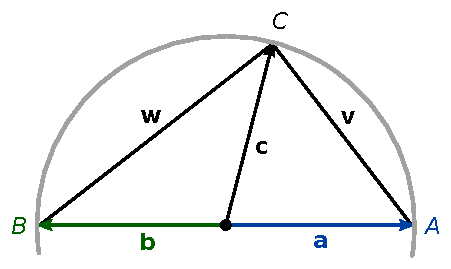
\includegraphics{img/Thales.pdf}
\caption{Zeichnung zum Satz des Thales}
\end{figure}

\begin{figure}[b!]
\centering
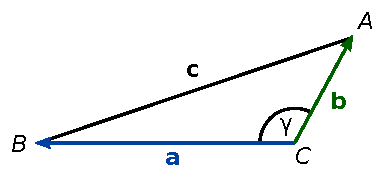
\includegraphics{img/Kosinussatz.pdf}
\caption{Zeichnung zum Kosinussatz}
\end{figure}

\newpage
\begin{Satz}[Sinussatz]
Für jedes Dreieck $\triangle ABC$ gilt
\[\frac{a}{\sin\alpha} = \frac{b}{\sin\beta} = \frac{c}{\sin\gamma}
= \frac{abc}{2A},\]
wobei $A$ der Flächeninhalt ist.
\end{Satz}
\begin{Beweis}
Sei $\mathbf a := \overrightarrow{CB}$, $\mathbf b:= \overrightarrow{CA}$
und $\mathbf c := \mathbf a-\mathbf b$. Dann gilt
\begin{align*}
ab\sin\gamma\;\mathbf e_1\wedge\mathbf e_2 &= \mathbf b\wedge\mathbf a,\\
bc\sin\alpha\;\mathbf e_1\wedge\mathbf e_2 &= \mathbf c\wedge(-\mathbf b)
= \mathbf b\wedge\mathbf c = \mathbf b\wedge (\mathbf a-\mathbf b)
= \mathbf b\wedge\mathbf a,\\
ac\sin\beta\;\mathbf e_1\wedge\mathbf e_2 &= (-\mathbf a)\wedge (-\mathbf c)
= \mathbf a\wedge\mathbf c
= \mathbf a\wedge(\mathbf a-\mathbf b)
= -\mathbf a\wedge\mathbf b = \mathbf b\wedge\mathbf a
\end{align*}
und $\mathbf b\wedge\mathbf a = 2A\,\mathbf e_1\wedge\mathbf e_2$.
Demnach gilt
\[ab\sin\gamma = bc\sin\alpha = ac\sin\beta = 2A.\]
Umformung der Gleichung führt zur Behauptung.\;\qedsymbol
\end{Beweis}
